%%===========================================================%%
%%                                                           %%
%%              DEAD MATERIAL CORRECTION APPENDIX            %%
%%                                                           %%
%%===========================================================%%

\chapter{Dead material effect on TPC track reconstruction efficiency}\label{appendix:deadMaterial}
\begin{figure}[hb]
	\caption[The amount of lost $\pi^+$ due to the interaction with dead material in front of TPC as a function of $p_T$, $\eta$ and $z$-vertex in CD and SD]{The amount of lost $\pi^-$ due to the interaction with dead material in front of TPC in CD and SD MC samples. Each plot represents the fraction of lost $\pi^+$, $\delta\epsilon_{ TPC}$ ($z$-axis), as a function of true particle pseudorapidity $\eta$ ($y$-axis) and transverse momentum $p_{T}$ ($x$-axis) in single $z$-vertex bin.}\label{fig:dead_materialSDCD3Dpip}
	\centering
	\parbox{0.325\textwidth}{
		\centering
		\includegraphics[width=\linewidth,page=49]{graphics/systematicsEfficiency/deadMaterial/secondaries_Unbinned_SDCD_.pdf}\\
		\includegraphics[width=\linewidth,page=52]{graphics/systematicsEfficiency/deadMaterial/secondaries_Unbinned_SDCD_.pdf}\\
		\includegraphics[width=\linewidth,page=55]{graphics/systematicsEfficiency/deadMaterial/secondaries_Unbinned_SDCD_.pdf}\\
		\includegraphics[width=\linewidth,page=58]{graphics/systematicsEfficiency/deadMaterial/secondaries_Unbinned_SDCD_.pdf}\\
	}~
	\parbox{0.325\textwidth}{
		\centering
		\includegraphics[width=\linewidth,page=50]{graphics/systematicsEfficiency/deadMaterial/secondaries_Unbinned_SDCD_.pdf}\\
		\includegraphics[width=\linewidth,page=53]{graphics/systematicsEfficiency/deadMaterial/secondaries_Unbinned_SDCD_.pdf}\\
		\includegraphics[width=\linewidth,page=56]{graphics/systematicsEfficiency/deadMaterial/secondaries_Unbinned_SDCD_.pdf}\\
		\includegraphics[width=\linewidth,page=59]{graphics/systematicsEfficiency/deadMaterial/secondaries_Unbinned_SDCD_.pdf}
	}%
	\parbox{0.325\textwidth}{
		\centering
		\includegraphics[width=\linewidth,page=51]{graphics/systematicsEfficiency/deadMaterial/secondaries_Unbinned_SDCD_.pdf}\\
		\includegraphics[width=\linewidth,page=54]{graphics/systematicsEfficiency/deadMaterial/secondaries_Unbinned_SDCD_.pdf}\\
		\includegraphics[width=\linewidth,page=57]{graphics/systematicsEfficiency/deadMaterial/secondaries_Unbinned_SDCD_.pdf}\\
		\includegraphics[width=\linewidth,page=60]{graphics/systematicsEfficiency/deadMaterial/secondaries_Unbinned_SDCD_.pdf}
	}%
\end{figure}
\begin{figure}[H]\ContinuedFloat
	% ~\\[32pt]
	\parbox{0.325\textwidth}{
		\centering
		\includegraphics[width=\linewidth,page=61]{graphics/systematicsEfficiency/deadMaterial/secondaries_Unbinned_SDCD_.pdf}\\
	}~
	\parbox{0.325\textwidth}{
		\centering
		\includegraphics[width=\linewidth,page=62]{graphics/systematicsEfficiency/deadMaterial/secondaries_Unbinned_SDCD_.pdf}\\
	}
	\parbox{0.325\textwidth}{
		\centering
		\includegraphics[width=\linewidth,page=63]{graphics/systematicsEfficiency/deadMaterial/secondaries_Unbinned_SDCD_.pdf}\\
	}
\end{figure}
\begin{figure}[H]\ContinuedFloat
	% ~\\[32pt]
	%\centering
	\parbox{0.325\textwidth}{
		\centering
		\includegraphics[width=\linewidth,page=64]{graphics/systematicsEfficiency/deadMaterial/secondaries_Unbinned_SDCD_.pdf}\\
	}~
\end{figure}

%%%K-
\begin{figure}[H]
	\caption[The amount of lost $K^-$ due to the interaction with dead material in front of TPC as a function of $p_T$, $\eta$ and $z$-vertex in CD and SD]{The amount of lost $K^-$ due to the interaction with dead material in front of TPC in CD and SD MC samples. Each plot represents the fraction of lost $K^-$, $\delta\epsilon_{ TPC}$ ($z$-axis), as a function of true particle pseudorapidity $\eta$ ($y$-axis) and transverse momentum $p_{T}$ ($x$-axis) in single $z$-vertex bin.}\label{fig:dead_materialCDSD3DKm}
	\parbox{0.325\textwidth}{
		\includegraphics[width=\linewidth,page=17]{graphics/systematicsEfficiency/deadMaterial/secondaries_Unbinned_SDCD_.pdf}\\
		\includegraphics[width=\linewidth,page=20]{graphics/systematicsEfficiency/deadMaterial/secondaries_Unbinned_SDCD_.pdf}\\
		\includegraphics[width=\linewidth,page=23]{graphics/systematicsEfficiency/deadMaterial/secondaries_Unbinned_SDCD_.pdf}\\
		\includegraphics[width=\linewidth,page=26]{graphics/systematicsEfficiency/deadMaterial/secondaries_Unbinned_SDCD_.pdf}\\
		\includegraphics[width=\linewidth,page=29]{graphics/systematicsEfficiency/deadMaterial/secondaries_Unbinned_SDCD_.pdf}\\
	}~
	\parbox{0.325\textwidth}{
		\includegraphics[width=\linewidth,page=18]{graphics/systematicsEfficiency/deadMaterial/secondaries_Unbinned_SDCD_.pdf}\\
		\includegraphics[width=\linewidth,page=21]{graphics/systematicsEfficiency/deadMaterial/secondaries_Unbinned_SDCD_.pdf}\\
		\includegraphics[width=\linewidth,page=24]{graphics/systematicsEfficiency/deadMaterial/secondaries_Unbinned_SDCD_.pdf}\\
		\includegraphics[width=\linewidth,page=27]{graphics/systematicsEfficiency/deadMaterial/secondaries_Unbinned_SDCD_.pdf}
		\includegraphics[width=\linewidth,page=30]{graphics/systematicsEfficiency/deadMaterial/secondaries_Unbinned_SDCD_.pdf}\\
	}%
	\parbox{0.325\textwidth}{
		\includegraphics[width=\linewidth,page=19]{graphics/systematicsEfficiency/deadMaterial/secondaries_Unbinned_SDCD_.pdf}\\
		\includegraphics[width=\linewidth,page=22]{graphics/systematicsEfficiency/deadMaterial/secondaries_Unbinned_SDCD_.pdf}\\
		\includegraphics[width=\linewidth,page=25]{graphics/systematicsEfficiency/deadMaterial/secondaries_Unbinned_SDCD_.pdf}\\
		\includegraphics[width=\linewidth,page=28]{graphics/systematicsEfficiency/deadMaterial/secondaries_Unbinned_SDCD_.pdf}
		\includegraphics[width=\linewidth,page=31]{graphics/systematicsEfficiency/deadMaterial/secondaries_Unbinned_SDCD_.pdf}\\
	}%
\end{figure}

\begin{figure}[H]\ContinuedFloat
	% ~\\[32pt]
	\vspace{-3.5em}
	\parbox{0.325\textwidth}{
		\includegraphics[width=\linewidth,page=32]{graphics/systematicsEfficiency/deadMaterial/secondaries_Unbinned_SDCD_.pdf}\\
	}~
	\vspace{-4em}
\end{figure}
%%%K+
\begin{figure}[H]
	\caption[The amount of lost $K^+$ due to the interaction with dead material in front of TPC as a function of $p_T$, $\eta$ and $z$-vertex in CD and SD]{The amount of lost $K^+$ due to the interaction with dead material in front of TPC in CD and SD MC samples. Each plot represents the fraction of lost $K^+$, $\delta\epsilon_{ TPC}$ ($z$-axis), as a function of true particle pseudorapidity $\eta$ ($y$-axis) and transverse momentum $p_{T}$ ($x$-axis) in single $z$-vertex bin.}\label{fig:dead_materialCDSD3DKp}
	\parbox{0.325\textwidth}{
		\includegraphics[width=\linewidth,page=65]{graphics/systematicsEfficiency/deadMaterial/secondaries_Unbinned_SDCD_.pdf}\\
		\includegraphics[width=\linewidth,page=68]{graphics/systematicsEfficiency/deadMaterial/secondaries_Unbinned_SDCD_.pdf}\\
		\includegraphics[width=\linewidth,page=71]{graphics/systematicsEfficiency/deadMaterial/secondaries_Unbinned_SDCD_.pdf}\\
		\includegraphics[width=\linewidth,page=74]{graphics/systematicsEfficiency/deadMaterial/secondaries_Unbinned_SDCD_.pdf}\\
		\includegraphics[width=\linewidth,page=77]{graphics/systematicsEfficiency/deadMaterial/secondaries_Unbinned_SDCD_.pdf}\\
	}~
	\parbox{0.325\textwidth}{
		\includegraphics[width=\linewidth,page=66]{graphics/systematicsEfficiency/deadMaterial/secondaries_Unbinned_SDCD_.pdf}\\
		\includegraphics[width=\linewidth,page=69]{graphics/systematicsEfficiency/deadMaterial/secondaries_Unbinned_SDCD_.pdf}\\
		\includegraphics[width=\linewidth,page=72]{graphics/systematicsEfficiency/deadMaterial/secondaries_Unbinned_SDCD_.pdf}\\
		\includegraphics[width=\linewidth,page=75]{graphics/systematicsEfficiency/deadMaterial/secondaries_Unbinned_SDCD_.pdf}
		\includegraphics[width=\linewidth,page=78]{graphics/systematicsEfficiency/deadMaterial/secondaries_Unbinned_SDCD_.pdf}\\
	}%
	\parbox{0.325\textwidth}{
		\includegraphics[width=\linewidth,page=67]{graphics/systematicsEfficiency/deadMaterial/secondaries_Unbinned_SDCD_.pdf}\\
		\includegraphics[width=\linewidth,page=70]{graphics/systematicsEfficiency/deadMaterial/secondaries_Unbinned_SDCD_.pdf}\\
		\includegraphics[width=\linewidth,page=73]{graphics/systematicsEfficiency/deadMaterial/secondaries_Unbinned_SDCD_.pdf}\\
		\includegraphics[width=\linewidth,page=76]{graphics/systematicsEfficiency/deadMaterial/secondaries_Unbinned_SDCD_.pdf}
		\includegraphics[width=\linewidth,page=79]{graphics/systematicsEfficiency/deadMaterial/secondaries_Unbinned_SDCD_.pdf}\\
	}%
\end{figure}

\begin{figure}[H]\ContinuedFloat
	% ~\\[32pt]
	\vspace{-3.5em}
	\parbox{0.325\textwidth}{
		\includegraphics[width=\linewidth,page=80]{graphics/systematicsEfficiency/deadMaterial/secondaries_Unbinned_SDCD_.pdf}\\
	}~
	\vspace{-4em}
\end{figure}
%%%pbar
\begin{figure}[H]
	\caption[The amount of lost $\bar{p}$ due to the interaction with dead material in front of TPC as a function of $p_T$, $\eta$ and $z$-vertex in CD and SD]{The amount of lost $\bar{p}$ due to the interaction with dead material in front of TPC in CD and SD MC samples. Each plot represents the fraction of lost $\bar{p}$, $\delta\epsilon_{ TPC}$ ($z$-axis), as a function of true particle pseudorapidity $\eta$ ($y$-axis) and transverse momentum $p_{T}$ ($x$-axis) in single $z$-vertex bin.}\label{fig:dead_materialCDSD3Dpbar}
	\parbox{0.325\textwidth}{
		\includegraphics[width=\linewidth,page=33]{graphics/systematicsEfficiency/deadMaterial/secondaries_Unbinned_SDCD_.pdf}\\
		\includegraphics[width=\linewidth,page=36]{graphics/systematicsEfficiency/deadMaterial/secondaries_Unbinned_SDCD_.pdf}\\
		\includegraphics[width=\linewidth,page=39]{graphics/systematicsEfficiency/deadMaterial/secondaries_Unbinned_SDCD_.pdf}\\
		\includegraphics[width=\linewidth,page=42]{graphics/systematicsEfficiency/deadMaterial/secondaries_Unbinned_SDCD_.pdf}\\
		\includegraphics[width=\linewidth,page=45]{graphics/systematicsEfficiency/deadMaterial/secondaries_Unbinned_SDCD_.pdf}\\
	}~
	\parbox{0.325\textwidth}{
		\includegraphics[width=\linewidth,page=34]{graphics/systematicsEfficiency/deadMaterial/secondaries_Unbinned_SDCD_.pdf}\\
		\includegraphics[width=\linewidth,page=37]{graphics/systematicsEfficiency/deadMaterial/secondaries_Unbinned_SDCD_.pdf}\\
		\includegraphics[width=\linewidth,page=40]{graphics/systematicsEfficiency/deadMaterial/secondaries_Unbinned_SDCD_.pdf}\\
		\includegraphics[width=\linewidth,page=43]{graphics/systematicsEfficiency/deadMaterial/secondaries_Unbinned_SDCD_.pdf}
		\includegraphics[width=\linewidth,page=46]{graphics/systematicsEfficiency/deadMaterial/secondaries_Unbinned_SDCD_.pdf}\\
	}%
	\parbox{0.325\textwidth}{
		\includegraphics[width=\linewidth,page=35]{graphics/systematicsEfficiency/deadMaterial/secondaries_Unbinned_SDCD_.pdf}\\
		\includegraphics[width=\linewidth,page=38]{graphics/systematicsEfficiency/deadMaterial/secondaries_Unbinned_SDCD_.pdf}\\
		\includegraphics[width=\linewidth,page=41]{graphics/systematicsEfficiency/deadMaterial/secondaries_Unbinned_SDCD_.pdf}\\
		\includegraphics[width=\linewidth,page=44]{graphics/systematicsEfficiency/deadMaterial/secondaries_Unbinned_SDCD_.pdf}
		\includegraphics[width=\linewidth,page=47]{graphics/systematicsEfficiency/deadMaterial/secondaries_Unbinned_SDCD_.pdf}\\
	}%
\end{figure}

\begin{figure}[H]\ContinuedFloat
	% ~\\[32pt]
	\vspace{-3.5em}
	\parbox{0.325\textwidth}{
		\includegraphics[width=\linewidth,page=48]{graphics/systematicsEfficiency/deadMaterial/secondaries_Unbinned_SDCD_.pdf}\\
	}~
	\vspace{-4em}
\end{figure}
%%%p
\begin{figure}[H]
	\caption[The amount of lost $p$ due to the interaction with dead material in front of TPC as a function of $p_T$, $\eta$ and $z$-vertex in CD and SD]{The amount of lost $p$ due to the interaction with dead material in front of TPC in CD and SD MC samples. Each plot represents the fraction of lost $p$, $\delta\epsilon_{ TPC}$ ($z$-axis), as a function of true particle pseudorapidity $\eta$ ($y$-axis) and transverse momentum $p_{T}$ ($x$-axis) in single $z$-vertex bin.}\label{fig:dead_materialCDSD3Dp}
	\parbox{0.325\textwidth}{
		\includegraphics[width=\linewidth,page=81]{graphics/systematicsEfficiency/deadMaterial/secondaries_Unbinned_SDCD_.pdf}\\
		\includegraphics[width=\linewidth,page=84]{graphics/systematicsEfficiency/deadMaterial/secondaries_Unbinned_SDCD_.pdf}\\
		\includegraphics[width=\linewidth,page=87]{graphics/systematicsEfficiency/deadMaterial/secondaries_Unbinned_SDCD_.pdf}\\
		\includegraphics[width=\linewidth,page=90]{graphics/systematicsEfficiency/deadMaterial/secondaries_Unbinned_SDCD_.pdf}\\
		\includegraphics[width=\linewidth,page=93]{graphics/systematicsEfficiency/deadMaterial/secondaries_Unbinned_SDCD_.pdf}\\
	}~
	\parbox{0.325\textwidth}{
		\includegraphics[width=\linewidth,page=82]{graphics/systematicsEfficiency/deadMaterial/secondaries_Unbinned_SDCD_.pdf}\\
		\includegraphics[width=\linewidth,page=85]{graphics/systematicsEfficiency/deadMaterial/secondaries_Unbinned_SDCD_.pdf}\\
		\includegraphics[width=\linewidth,page=88]{graphics/systematicsEfficiency/deadMaterial/secondaries_Unbinned_SDCD_.pdf}\\
		\includegraphics[width=\linewidth,page=91]{graphics/systematicsEfficiency/deadMaterial/secondaries_Unbinned_SDCD_.pdf}
		\includegraphics[width=\linewidth,page=94]{graphics/systematicsEfficiency/deadMaterial/secondaries_Unbinned_SDCD_.pdf}\\
	}%
	\parbox{0.325\textwidth}{
		\includegraphics[width=\linewidth,page=83]{graphics/systematicsEfficiency/deadMaterial/secondaries_Unbinned_SDCD_.pdf}\\
		\includegraphics[width=\linewidth,page=86]{graphics/systematicsEfficiency/deadMaterial/secondaries_Unbinned_SDCD_.pdf}\\
		\includegraphics[width=\linewidth,page=89]{graphics/systematicsEfficiency/deadMaterial/secondaries_Unbinned_SDCD_.pdf}\\
		\includegraphics[width=\linewidth,page=92]{graphics/systematicsEfficiency/deadMaterial/secondaries_Unbinned_SDCD_.pdf}
		\includegraphics[width=\linewidth,page=95]{graphics/systematicsEfficiency/deadMaterial/secondaries_Unbinned_SDCD_.pdf}\\
	}%
\end{figure}

\begin{figure}[H]\ContinuedFloat
	% ~\\[32pt]
	\vspace{-3.5em}
	\parbox{0.325\textwidth}{
		\includegraphics[width=\linewidth,page=96]{graphics/systematicsEfficiency/deadMaterial/secondaries_Unbinned_SDCD_.pdf}\\
	}~
	\vspace{-4em}
\end{figure}
%%%negative
\begin{figure}[H]
	\caption[The amount of lost negative particles due to the interaction with dead material in front of TPC as a function of $p_T$, $\eta$ and $z$-vertex in CD and SD]{The amount of lost negative particles due to the interaction with dead material in front of TPC in CD and SD MC samples. Each plot represents the fraction of lost negative particles, $\delta\epsilon_{ TPC}$ ($z$-axis), as a function of true particle pseudorapidity $\eta$ ($y$-axis) and transverse momentum $p_{T}$ ($x$-axis) in single $z$-vertex bin.}\label{fig:dead_materialCDSD3Dnegative}
	\parbox{0.325\textwidth}{
		\includegraphics[width=\linewidth,page=1]{graphics/systematicsEfficiency/deadMaterial/secondaries_Unbinned_Charged_SDCD.pdf}\\
		\includegraphics[width=\linewidth,page=4]{graphics/systematicsEfficiency/deadMaterial/secondaries_Unbinned_Charged_SDCD.pdf}\\
		\includegraphics[width=\linewidth,page=7]{graphics/systematicsEfficiency/deadMaterial/secondaries_Unbinned_Charged_SDCD.pdf}\\
		\includegraphics[width=\linewidth,page=10]{graphics/systematicsEfficiency/deadMaterial/secondaries_Unbinned_Charged_SDCD.pdf}\\
		\includegraphics[width=\linewidth,page=13]{graphics/systematicsEfficiency/deadMaterial/secondaries_Unbinned_Charged_SDCD.pdf}\\
	}~
	\parbox{0.325\textwidth}{
		\includegraphics[width=\linewidth,page=2]{graphics/systematicsEfficiency/deadMaterial/secondaries_Unbinned_Charged_SDCD.pdf}\\
		\includegraphics[width=\linewidth,page=5]{graphics/systematicsEfficiency/deadMaterial/secondaries_Unbinned_Charged_SDCD.pdf}\\
		\includegraphics[width=\linewidth,page=8]{graphics/systematicsEfficiency/deadMaterial/secondaries_Unbinned_Charged_SDCD.pdf}\\
		\includegraphics[width=\linewidth,page=11]{graphics/systematicsEfficiency/deadMaterial/secondaries_Unbinned_Charged_SDCD.pdf}
		\includegraphics[width=\linewidth,page=14]{graphics/systematicsEfficiency/deadMaterial/secondaries_Unbinned_Charged_SDCD.pdf}\\
	}%
	\parbox{0.325\textwidth}{
		\includegraphics[width=\linewidth,page=3]{graphics/systematicsEfficiency/deadMaterial/secondaries_Unbinned_Charged_SDCD.pdf}\\
		\includegraphics[width=\linewidth,page=6]{graphics/systematicsEfficiency/deadMaterial/secondaries_Unbinned_Charged_SDCD.pdf}\\
		\includegraphics[width=\linewidth,page=9]{graphics/systematicsEfficiency/deadMaterial/secondaries_Unbinned_Charged_SDCD.pdf}\\
		\includegraphics[width=\linewidth,page=12]{graphics/systematicsEfficiency/deadMaterial/secondaries_Unbinned_Charged_SDCD.pdf}
		\includegraphics[width=\linewidth,page=15]{graphics/systematicsEfficiency/deadMaterial/secondaries_Unbinned_Charged_SDCD.pdf}\\
	}%
\end{figure}

\begin{figure}[H]\ContinuedFloat
	% ~\\[32pt]
	\vspace{-3.5em}
	\parbox{0.325\textwidth}{
		\includegraphics[width=\linewidth,page=16]{graphics/systematicsEfficiency/deadMaterial/secondaries_Unbinned_Charged_SDCD.pdf}\\
	}~
	\vspace{-4em}
\end{figure}
%%%positive
\begin{figure}[H]
	\caption[The amount of lost positive particles due to the interaction with dead material in front of TPC as a function of $p_T$, $\eta$ and $z$-vertex in CD and SD]{The amount of lost positive particles due to the interaction with dead material in front of TPC in CD and SD MC samples. Each plot represents the fraction of lost positive particles, $\delta\epsilon_{ TPC}$ ($z$-axis), as a function of true particle pseudorapidity $\eta$ ($y$-axis) and transverse momentum $p_{T}$ ($x$-axis) in single $z$-vertex bin.}\label{fig:dead_materialCDSD3Dpositive}
	\parbox{0.325\textwidth}{
		\includegraphics[width=\linewidth,page=17]{graphics/systematicsEfficiency/deadMaterial/secondaries_Unbinned_Charged_SDCD.pdf}\\
		\includegraphics[width=\linewidth,page=20]{graphics/systematicsEfficiency/deadMaterial/secondaries_Unbinned_Charged_SDCD.pdf}\\
		\includegraphics[width=\linewidth,page=23]{graphics/systematicsEfficiency/deadMaterial/secondaries_Unbinned_Charged_SDCD.pdf}\\
		\includegraphics[width=\linewidth,page=26]{graphics/systematicsEfficiency/deadMaterial/secondaries_Unbinned_Charged_SDCD.pdf}\\
		\includegraphics[width=\linewidth,page=29]{graphics/systematicsEfficiency/deadMaterial/secondaries_Unbinned_Charged_SDCD.pdf}\\
	}~
	\parbox{0.325\textwidth}{
		\includegraphics[width=\linewidth,page=18]{graphics/systematicsEfficiency/deadMaterial/secondaries_Unbinned_Charged_SDCD.pdf}\\
		\includegraphics[width=\linewidth,page=21]{graphics/systematicsEfficiency/deadMaterial/secondaries_Unbinned_Charged_SDCD.pdf}\\
		\includegraphics[width=\linewidth,page=24]{graphics/systematicsEfficiency/deadMaterial/secondaries_Unbinned_Charged_SDCD.pdf}\\
		\includegraphics[width=\linewidth,page=27]{graphics/systematicsEfficiency/deadMaterial/secondaries_Unbinned_Charged_SDCD.pdf}
		\includegraphics[width=\linewidth,page=30]{graphics/systematicsEfficiency/deadMaterial/secondaries_Unbinned_Charged_SDCD.pdf}\\
	}%
	\parbox{0.325\textwidth}{
		\includegraphics[width=\linewidth,page=19]{graphics/systematicsEfficiency/deadMaterial/secondaries_Unbinned_Charged_SDCD.pdf}\\
		\includegraphics[width=\linewidth,page=22]{graphics/systematicsEfficiency/deadMaterial/secondaries_Unbinned_Charged_SDCD.pdf}\\
		\includegraphics[width=\linewidth,page=25]{graphics/systematicsEfficiency/deadMaterial/secondaries_Unbinned_Charged_SDCD.pdf}\\
		\includegraphics[width=\linewidth,page=28]{graphics/systematicsEfficiency/deadMaterial/secondaries_Unbinned_Charged_SDCD.pdf}
		\includegraphics[width=\linewidth,page=31]{graphics/systematicsEfficiency/deadMaterial/secondaries_Unbinned_Charged_SDCD.pdf}\\
	}%
\end{figure}

\begin{figure}[H]\ContinuedFloat
	% ~\\[32pt]
	\vspace{-3.5em}
	\parbox{0.325\textwidth}{
		\includegraphics[width=\linewidth,page=32]{graphics/systematicsEfficiency/deadMaterial/secondaries_Unbinned_Charged_SDCD.pdf}\\
	}~
	\vspace{-4em}
\end{figure}